\subsubsection{傾斜センサー}\label{tilt}
\begin{table}[H]
  \begin{widerrows}
    \begin{tabular}{|p{\colF}|p{\colG}|}	\hline
    名称 & 傾斜センサー(けいしゃせんさー)\\ \hline
    接続箇所 & デジタルコネクタ (3pin)\\ \hline
    機能概要 & 中のボールの転がりで、傾きを検知する\\ \hline
    \end{tabular}
  \end{widerrows} 
\end{table}

\begin{table}[H]
  \begin{widerrows}
    \begin{tabular}{|p{\colF}|p{\colG}|}	\hline
    サンプルコードの場所 & 05/digin.hsp\\ \hline
    raspiへの入力 & センサーが傾くと1、傾いていないと0の値を入力します。\\ \hline
    raspiへの入力方法 & val = gpioin(GPIO番号)\\ \hline
    raspiからの出力 & なし\\ \hline
    raspiからの出力方法 & なし\\ \hline
    \end{tabular}
  \end{widerrows} 
\end{table}

\begin{figure}[H]
  \begin{widerrows}
    \begin{tabular}{|p{\colF}|p{\colG}|} \hline
    使い道 & ストーブの安全装置\\ \hline
    注意事項 & なし\\ \hline
    補足 & 黒い箱のなかにボールが入っていて、ボールが転がり\ruby{端子}{たん|し}に\ruby{触}{ふ}れるとONになります。傾いていないときはOFFになります。
    \par
    \begin{minipage}[t]{\linewidth}
      \smallskip
        \centering
        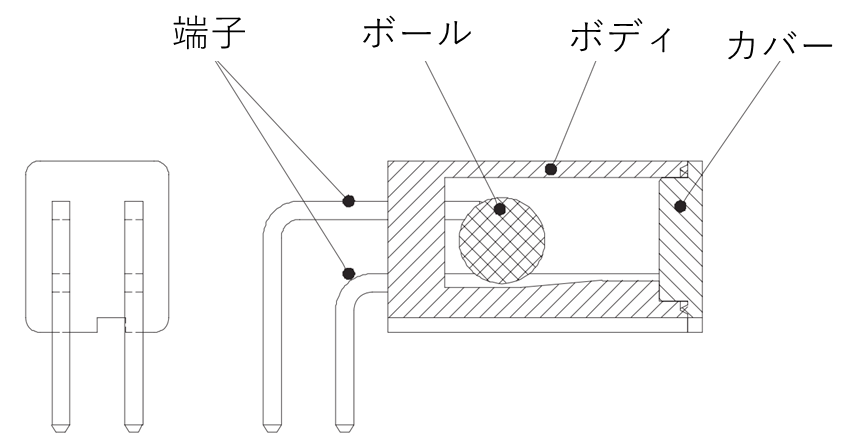
\includegraphics[width=0.7\linewidth]{images/chap05/text05-img046.png}
        \caption{傾斜センサーの内部}
        \smallskip
      \end{minipage}
    \\ \hline
    \end{tabular}
  \end{widerrows} 
\end{figure}

\begin{figure}[H]
  \begin{widerrows}
    \begin{tabular}{|p{\colH}|p{\colI}|p{\colH}|p{\colI}|} \hline
    外観 & 
    \begin{minipage}[t]{\linewidth}
      \smallskip
        \centering
        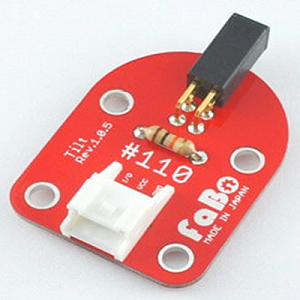
\includegraphics[width=0.5\linewidth]{images/chap05/text05-img018.png}
        \caption{傾斜センサー}
        \smallskip
      \end{minipage} &
      回路記号 & 
      \begin{minipage}[t]{\linewidth}
      \smallskip
        \centering
        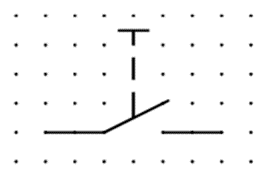
\includegraphics[width=0.5\linewidth]{images/chap05/text05-img047.png}
        \caption{傾斜センサーの回路図}
        \smallskip
      \end{minipage}\\ \hline
    \end{tabular}
  \end{widerrows} 
\end{figure}